     %%%%%%%%%%%%%%%%%%%%
     %                                                   %
     %  capitolo1.tex   %
     %                  %
     %%%%%%%%%%%%%%%%%%%%

\section{Esperimenti}\label{sec:esperimenti}

Abbiamo provato il nostro software su tre diversi video. Tutti e tre sono filmati in cui la camera è fissa e c'è un singolo oggetto in movimento, che può sia uscire dall'inquadratura che nascondersi dietro qualche oggetto all'interno della scena (occlusione). In tutti e tre nei primi frames  non compare alcun oggetto in moto, questo per facilitare il Background Subtraction.\\

Per ciascun video abbiamo osservato/confrontato il comportamento dei due filtri al variare di alcuni parametri quali:
\begin{itemize}
\item frequenza di campionamento (MOD)
\item covarianza relativa al rumore del processo studiato (Q), che stabilisce la tolleranza consentita alla predizione di Kalman
\item numero di campioni utilizzati dal Condensation\\
\end{itemize}

I risultati prodotti per ciascuna prova sono rappresentati in due grafici:
\begin{itemize}
\item Il primo rappresenta per ogni campionamento:
\begin{itemize}
\item la posizione dell'oggetto
\item la posizione predetta dal filtro di Kalman
\item la posizione predetta dal Condensation
\end{itemize}
\item Il secondo rappresenta quanto rispettivamente ciascuna predizione si discosta dalla posizione reale dell'oggetto.
\end{itemize}


Abbiamo provato il nostro software su tre diversi video. Tutti e tre sono filmati in cui la camera è fissa e c'è un singolo oggetto in movimento, che può sia uscire dall'inquadratura che nascondersi dietro qualche oggetto all'interno della scena (occlusione). In tutti e tre nei primi frames  non compare alcun oggetto in moto, questo per facilitare il Background Subtraction.\\

Per ciascun video abbiamo osservato/confrontato il comportamento dei due filtri al variare di alcuni parametri quali:
\begin{itemize}
\item frequenza di campionamento (MOD)
\item covarianza relativa al rumore del processo studiato (Q), che stabilisce la tolleranza consentita alla predizione di Kalman
\item numero di campioni utilizzati dal Condensation\\
\end{itemize}

I risultati prodotti per ciascuna prova sono rappresentati in due grafici:
\begin{itemize}
\item Il primo rappresenta per ogni campionamento:
\begin{itemize}
\item la posizione dell'oggetto
\item la posizione predetta dal filtro di Kalman
\item la posizione predetta dal Condensation
\end{itemize}
\item Il secondo rappresenta quanto rispettivamente ciascuna predizione si discosta dalla posizione reale dell'oggetto.
\end{itemize}

Inoltre per ogni test viene dato il valore medio della distanza tra posizione predetta e posizione reale per i due filtri \begin{math}(\bar \delta_K, \bar \delta_C)\end{math}, oltre al valore della varianza media per il Condensation \begin{math}(\sigma_x,\sigma_y)\end{math}.


Inoltre per ogni test viene dato il valore medio della distanza tra posizione predetta e posizione reale per i due filtri \begin{math}(\bar \delta_K, \bar \delta_C)\end{math}, oltre al valore della varianza media per il Condensation \begin{math}(\sigma_x,\sigma_y)\end{math}.


\newpage

\subsection{Video: movies12.mjpeg}
\begin{itemize}
\item risoluzione: 640x480
\item fps: 25.00
\item durata: 50.4 s
\end{itemize}


Si tratta di una ripresa trasversale dall'alto di un automobilina radiocomandata. In questa scena i punti di occlusione sono due: una scatola al centro della scena e un ostacolo sulla sinistra. La macchina non subisce repentine accelerazioni o decelerazioni, in generale ruota attorno alla scatola centrale e riamane nascosta diestro questa per un po'. L'automobilina non esce mai dalla scena.

\begin{figure}[hb]
\centering
	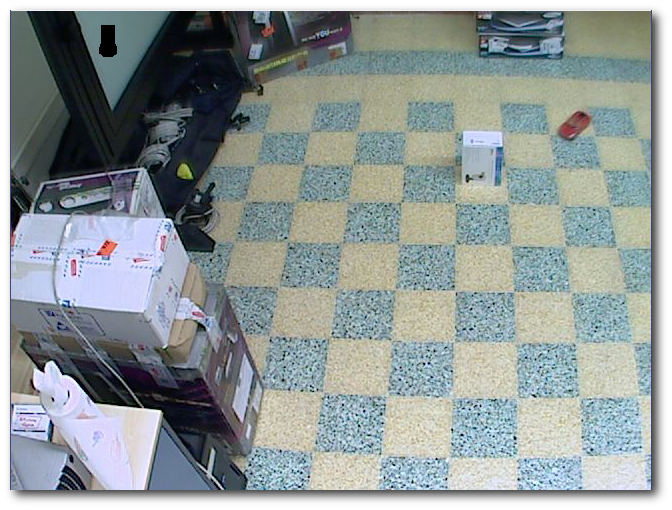
\includegraphics[scale=0.5]{movie12.png}
\caption{\textit{movie12 screenshot}}
\end{figure}
 
\newpage

Si tratta di una ripresa trasversale dall'alto di un automobilina radiocomandata. In questa scena i punti di occlusione sono due: una scatola al centro della scena e un ostacolo sulla sinistra. La macchina non subisce repentine accelerazioni o decelerazioni, in generale ruota attorno alla scatola centrale e riamane nascosta diestro questa per un po'. L'automobilina non esce mai dalla scena.

\begin{figure}[hb]
\centering
	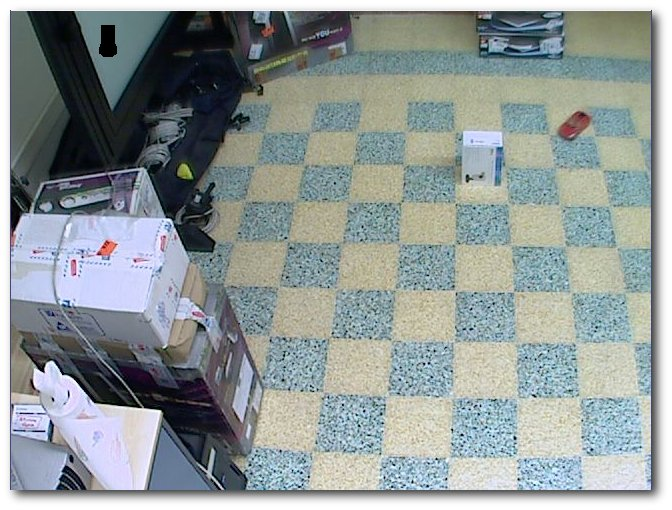
\includegraphics[scale=0.5]{movie12.jpg}
\caption{\textit{movie12 screenshot}}
\end{figure}
 
\newpage
\subsubsection{Test 1: MOD=3 , Q=1000, S=1000}

\begin{figure}[hb]
\centering
	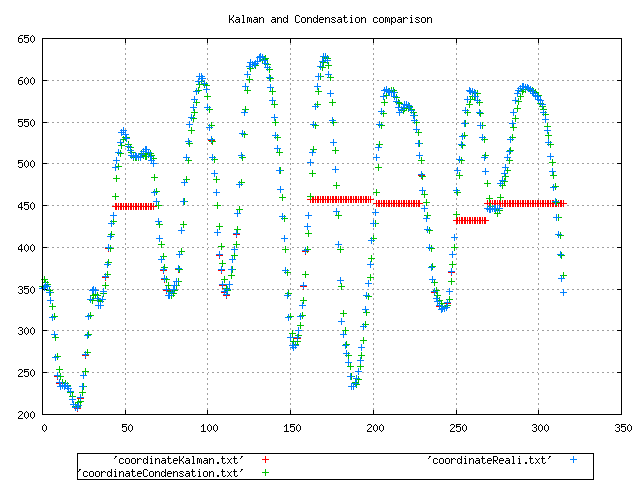
\includegraphics[scale=0.4]{../../esperimenti/movie12/mod_3-Q_1000-S_1000/plot.png}
\caption{\textit{Test 1: Tracciamento}}
\end{figure}

\begin{figure}[hb]
\centering
	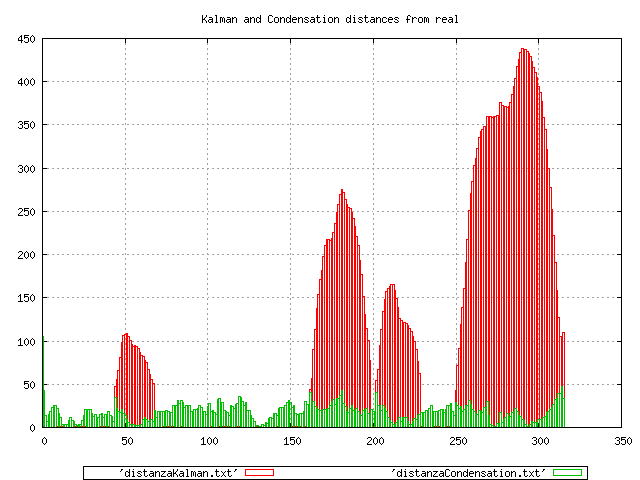
\includegraphics[scale=0.4]{../../esperimenti/movie12/mod_3-Q_1000-S_1000/plot-distances.png}
\caption{\textit{Test 1: Previsioni}}
\end{figure}

Statistiche:
\begin{itemize}
\item \begin{math} \bar \delta_K: 105 \end{math}
\item \begin{math} \bar \delta_C: 18 \end{math}
\item \begin{math}(\sigma_x,\sigma_y)\end{math}: (112,81)
\end{itemize}

Con queste impostazioni la dimensione dell'area di confidenza per Kalman non è sufficiente per mantenere traccia dell'oggetto, se viene persa una misurazione a causa dell'occlusione. Questo avviene ogni volta che l'oggetto viene nascosto, tuttavia non appena l'oggetto ripassa vicino a dove kalman si è fermato questo ricomincia ad essere tracciato correttamente. A differenza di kalman il condenstaion non perde mai l'oggetto, ma la stima del moto è decisamente meno precisa rispetto a quella effettuata dal filtro di kalman.

\newpage

\subsubsection{Test 2: MOD=3, Q=2000, S=1000}

\begin{figure}[hb]
\centering
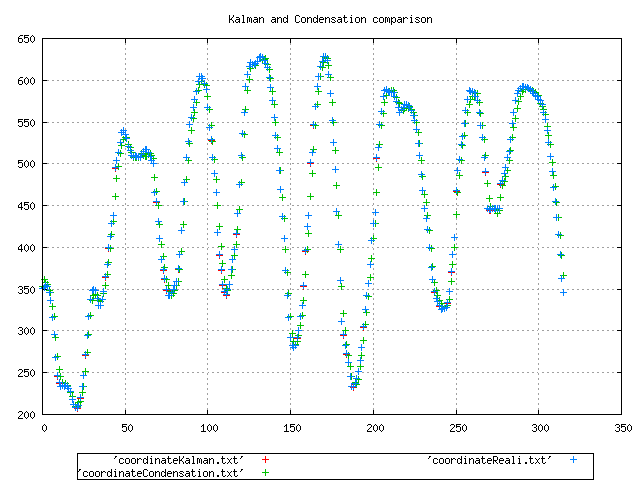
\includegraphics[scale=0.4]{../../esperimenti/movie12/mod_3-Q_2000-S_1000/plot.png}
\caption{\textit{Test 2: Tracciamento}}
\end{figure}

\begin{figure}[hb]
\centering
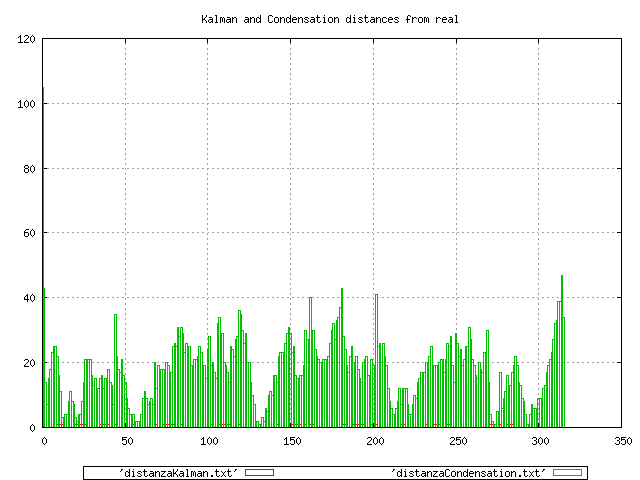
\includegraphics[scale=0.4]{../../esperimenti/movie12/mod_3-Q_2000-S_1000/plot-distances.png}
\caption{\textit{Test 2: Previsioni}}
\end{figure}

Statistiche:
\begin{itemize}
\item \begin{math} \bar \delta_K: 0 \end{math}
\item \begin{math} \bar \delta_C: 18 \end{math}
\item \begin{math}(\sigma_x,\sigma_y)\end{math}: (112,81)
\end{itemize}

Allargando l'area di confidenza per kalaman l'oggetto non viene mai perso e il tracciamento può essere valutato pressochè perfetto. Il comportamrento in questo caso è evidentemente migliore del Condesation.

\newpage
\subsubsection{Test 3: MOD=3, Q=1000, S=5000}

\begin{figure}[hb]
\centering
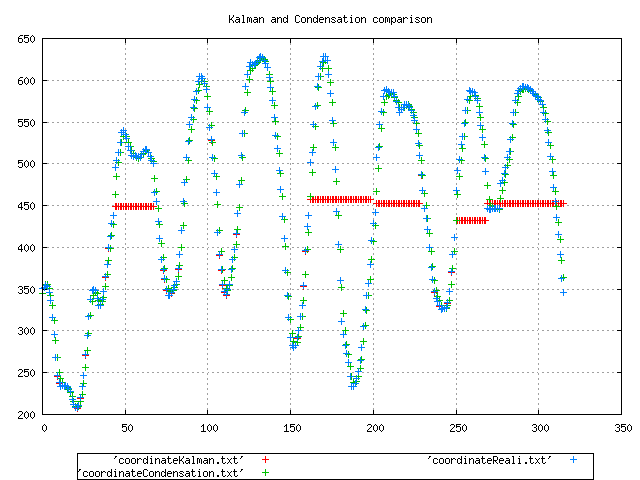
\includegraphics[scale=0.4]{../../esperimenti/movie12/mod_3-Q_1000-S_5000/plot.png}
\caption{\textit{Test 3: Tracciamento}}
\end{figure}

\begin{figure}[hb]
\centering
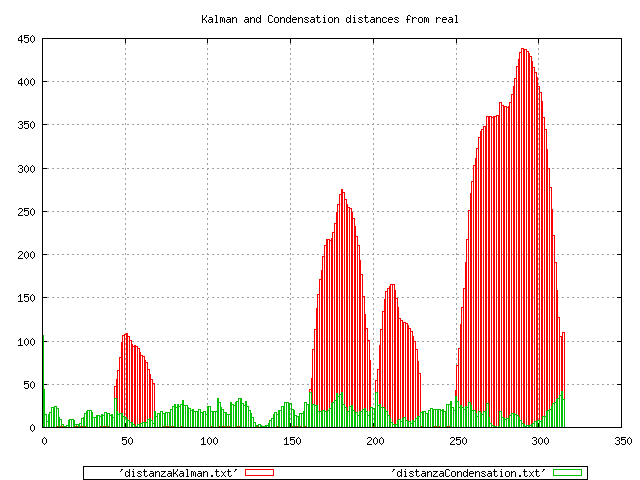
\includegraphics[scale=0.4]{../../esperimenti/movie12/mod_3-Q_1000-S_5000/plot-distances.png}
\caption{\textit{Test 3: Previsioni}}
\end{figure}

Statistiche:
\begin{itemize}
\item \begin{math} \bar \delta_K: 105 \end{math}
\item \begin{math} \bar \delta_C: 17 \end{math}
\item \begin{math}(\sigma_x,\sigma_y)\end{math}: (109,81)
\end{itemize}

Aumentando il numero di samples per il condenstaion abbiamo voluto valutare come  si comporta modificando le condizioni del primo test. Confrontando i risulati sulla previsione del solo condesantion nei due casi si vede che uno considerevole aumento del numero di sample da 1000 a 5000 porta non porta in media alcun miglioramento.

\newpage
\subsubsection{Test 4: MOD=3, Q=1000, S=100}

\begin{figure}[hb]
\centering
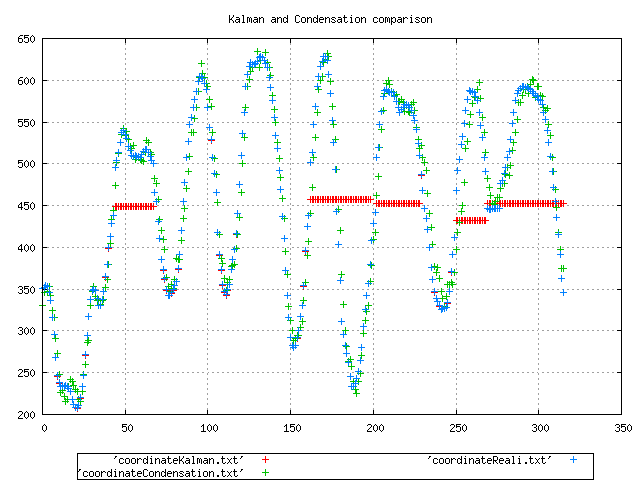
\includegraphics[scale=0.4]{../../esperimenti/movie12/mod_3-Q_1000-S_100/plot.png}
\caption{\textit{Test 4: Tracciamento}}
\end{figure}

\begin{figure}[hb]
\centering
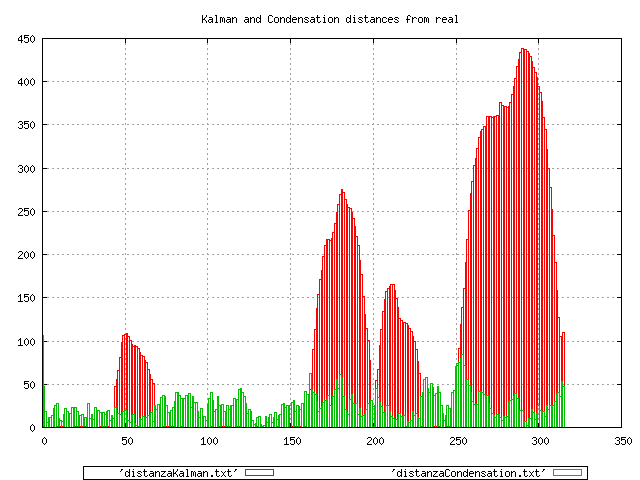
\includegraphics[scale=0.4]{../../esperimenti/movie12/mod_3-Q_1000-S_100/plot-distances.png}
\caption{\textit{Test 4: Previsioni}}
\end{figure}

Statistiche:
\begin{itemize}
\item \begin{math} \bar \delta_K: 105 \end{math}
\item \begin{math} \bar \delta_C: 24 \end{math}
\item \begin{math}(\sigma_x,\sigma_y)\end{math}: (140,92)
\end{itemize}


Il risutalto  per il condensation passando da 1000 a 100 sample invece è notevolemnte diverso. La stima del moto come si vede dal grafico è notevolemente peggiore nel secondo caso.

\newpage
\subsubsection{Test 5: MOD=3, Q=1000, S=10}

\begin{figure}[hb]
\centering
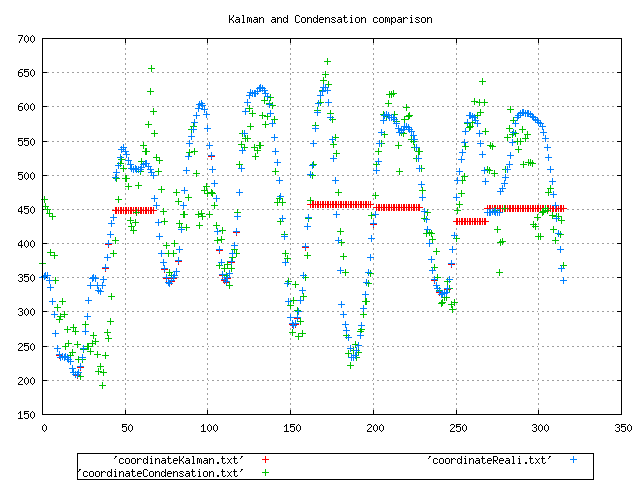
\includegraphics[scale=0.4]{../../esperimenti/movie12/mod_3-Q_1000-S_10/plot.png}
\caption{\textit{Test 5: Tracciamento}}
\end{figure}

\begin{figure}[hb]
\centering
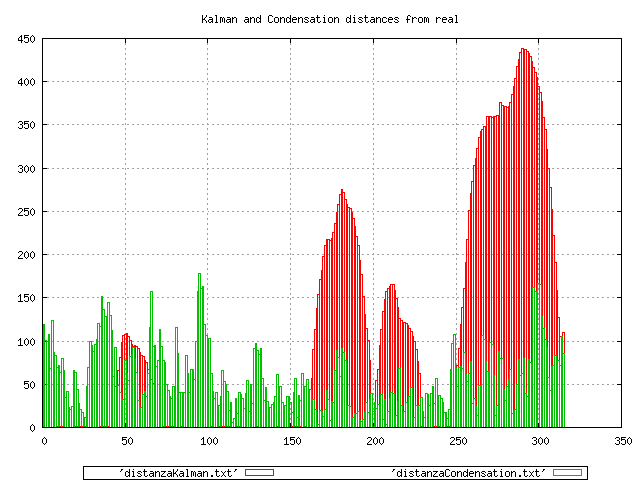
\includegraphics[scale=0.4]{../../esperimenti/movie12/mod_3-Q_1000-S_10/plot-distances.png}
\caption{\textit{Test 5: Previsioni}}
\end{figure}

Statistiche:
\begin{itemize}
\item \begin{math} \bar \delta_K: 105 \end{math}
\item \begin{math} \bar \delta_C: 55 \end{math}
\item \begin{math}(\sigma_x,\sigma_y)\end{math}: (195,112)
\end{itemize}


Proseguendo nel diminuire il numero di samples per il condensation siamo passati a 10, il confronto tra il caso in cui i sample sono 1000 è chiaramento mostrato nel grafico seguente. La previsione è notevolemente peggiore e addirittura si può dire che mediamente con 10 samples il condens. si comporta quasi come kalman  che perde l'oggetto. Come ci si poteva aspettare in condizioni estreme di lavoro le previsioni sono decisamente inattendibili.

\newpage
\subsection{Video: tappetonomod.avi}

\begin{itemize}
\item risoluzione: 320x240
\item fps: 10.00
\item durata: 60 s
\end{itemize}

Si tratta di una ripresa trasversale dall'alto. L'oggetto in movimento è un'automobilina radiocomandata che si muove su un'area delimitata da un tappeto. Il moto dell'automobilina subisce repentine accelerazioni e decelerazioni. Non ci sono oggetti occludenti, ma l'automobilina entra ed esce totalmente o parzialmente più di una volta dalla scena.

\begin{figure}[hb]
\centering
	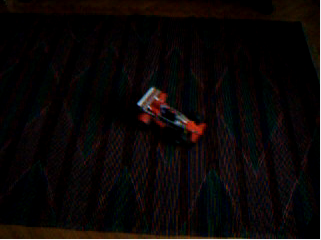
\includegraphics[scale=0.5]{tappeto_nomod.png}
\caption{\textit{tappeto-nomod screenshot}}
\end{figure}

\newpage
\subsubsection{Test 6: MOD=3, Q=1000, S=1000}

\begin{figure}[hb]
\centering
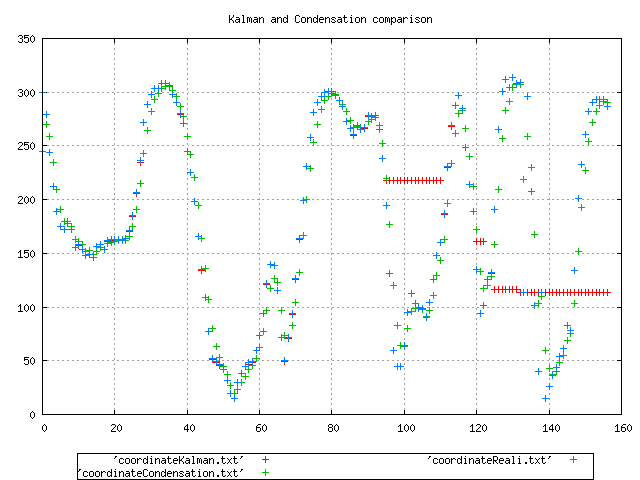
\includegraphics[scale=0.4]{../../esperimenti/tappeto_nozoom/mod_3-Q_1000-S_1000/plot.png}
\caption{\textit{Test 6: Tracciamento}}
\end{figure}

\begin{figure}[hb]
\centering
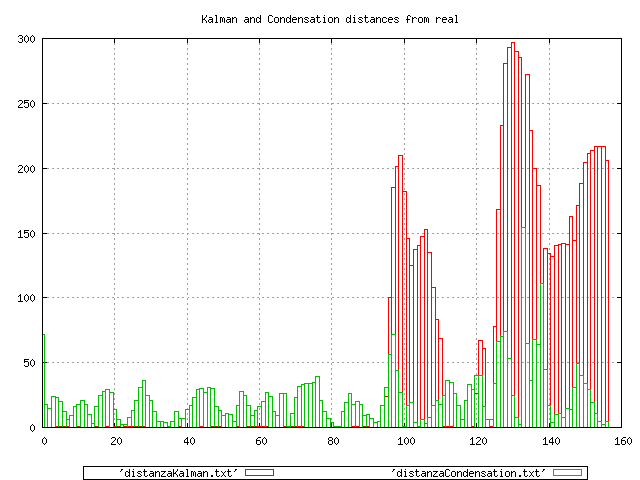
\includegraphics[scale=0.4]{../../esperimenti/tappeto_nozoom/mod_3-Q_1000-S_1000/plot-distances.png}
\caption{\textit{Test 6: Previsioni}}
\end{figure}

Statistiche:
\begin{itemize}
\item \begin{math} \bar \delta_K: 53 \end{math}
\item \begin{math} \bar \delta_C: 22 \end{math}
\item \begin{math}(\sigma_x,\sigma_y)\end{math}: (53,22)
\end{itemize}

La macchinina si sposta in modo molto rapido. Kalman si comporta in modo egregio fintato che l'oggetto si trova nell'inquadratura e che l'accelerazione della macchina non è tale da far uscire l'oggetto dall'area di previsione.

\newpage
\subsubsection{Test 7: MOD=5, Q=1000, S=1000}

\begin{figure}[hb]
\centering
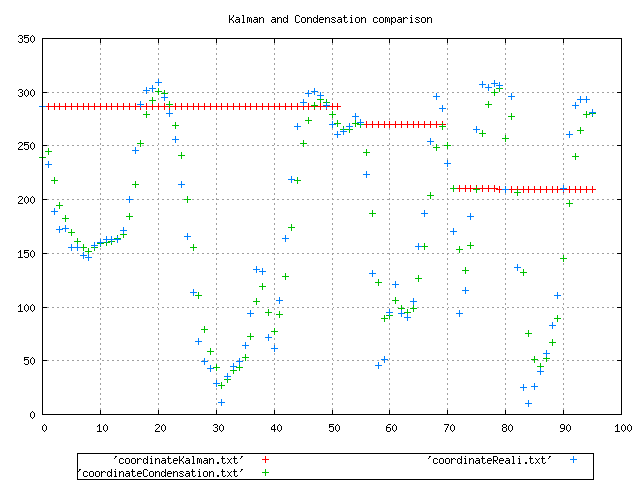
\includegraphics[scale=0.4]{../../esperimenti/tappeto_nozoom/mod_5-Q_1000-S_1000/plot.png}
\caption{\textit{Test 7: Tracciamento}}
\end{figure}

\begin{figure}[hb]
\centering
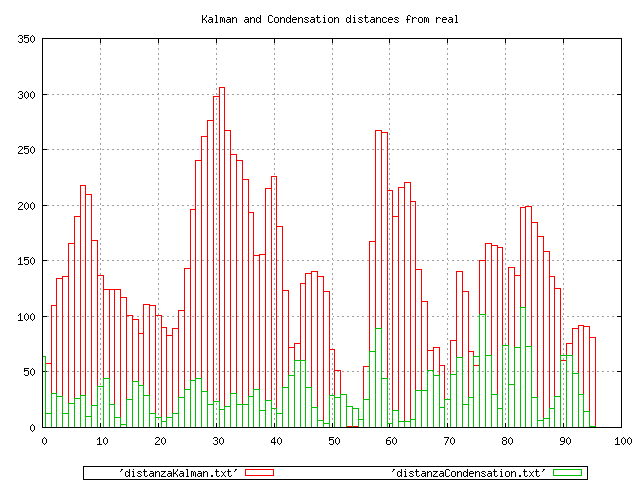
\includegraphics[scale=0.4]{../../esperimenti/tappeto_nozoom/mod_5-Q_1000-S_1000/plot-distances.png}
\caption{\textit{Test 7: Previsioni}}
\end{figure}

Statistiche:
\begin{itemize}
\item \begin{math} \bar \delta_K: 137 \end{math}
\item \begin{math} \bar \delta_C: 31\end{math}
\item \begin{math}(\sigma_x,\sigma_y)\end{math}: (56,40)
\end{itemize} 

Come prevedibile la rapidità di moto di questo oggetto mal si concilia una misurazione effettuata ad intervalli ampi. Entrambi i filtri si comportano in modo non proprio efficiente e perdono quasi immediatamente l'oggetto.

\newpage
\subsubsection{Test 8: MOD=2, Q=1000, S=1000}

\begin{figure}[hb]
\centering
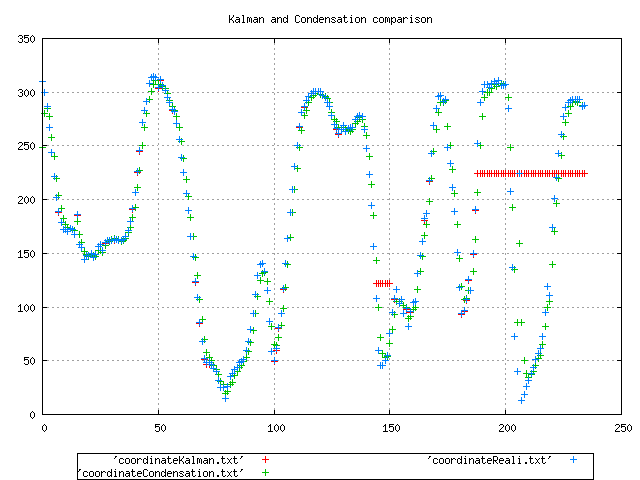
\includegraphics[scale=0.4]{../../esperimenti/tappeto_nozoom/mod_2-Q_1000-S_1000/plot.png}
\caption{\textit{Test 8: Tracciamento}}
\end{figure}

\begin{figure}[hb]
\centering
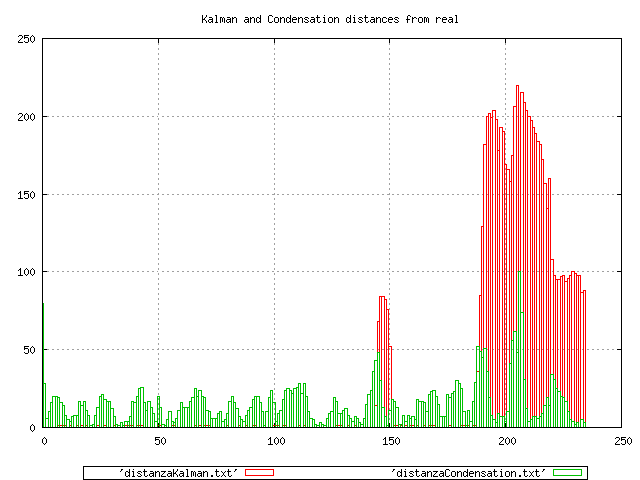
\includegraphics[scale=0.4]{../../esperimenti/tappeto_nozoom/mod_2-Q_1000-S_1000/plot-distances.png}
\caption{\textit{Test 8: Previsioni}}
\end{figure}

Statistiche:
\begin{itemize}
\item \begin{math} \bar \delta_K: 32 \end{math}
\item \begin{math} \bar \delta_C: 15 \end{math}
\item \begin{math}(\sigma_x,\sigma_y)\end{math}: (55,41)
\end{itemize}

La situazione decisamente migliora se invece campioniamo ogni 2 frames. Kalman fintato che non perde l'oggetto si comporta decisamente meglio del Condensation, in media però il Condensation risulta migliore.


\newpage
\subsubsection{Test 9: MOD=1, Q=2000, S=1000}

\begin{figure}[hb]
\centering
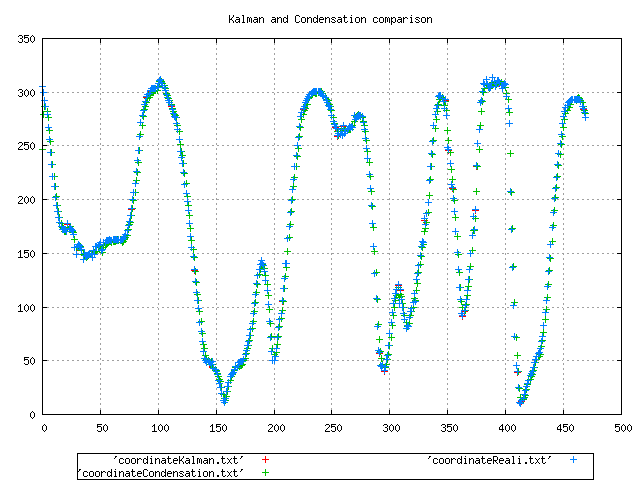
\includegraphics[scale=0.4]{../../esperimenti/tappeto_nozoom/mod_1-Q_2000-S_1000/plot.png}
\caption{\textit{Test 9: Tracciamento}}
\end{figure}

\begin{figure}[hb]
\centering
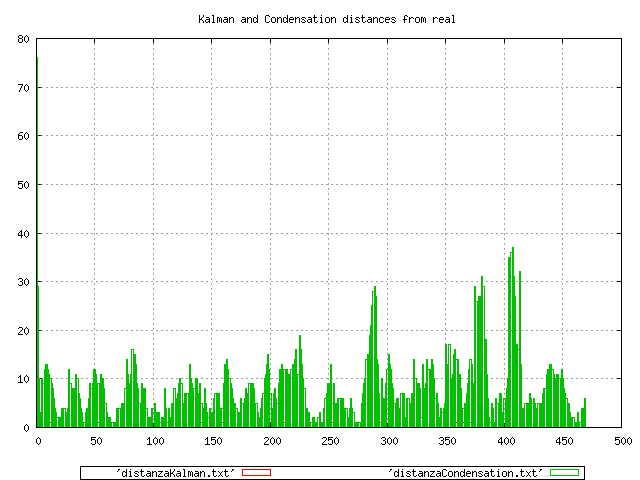
\includegraphics[scale=0.4]{../../esperimenti/tappeto_nozoom/mod_1-Q_2000-S_1000/plot-distances.png}
\caption{\textit{Test 9: Previsioni}}
\end{figure}

Statistiche:
\begin{itemize}
\item \begin{math} \bar \delta_K: 0 \end{math}
\item \begin{math} \bar \delta_C: 8 \end{math}
\item \begin{math}(\sigma_x,\sigma_y)\end{math}: (55,41)
\end{itemize}

Ingrandendo l'area di tolleranza per Kalman e prendendo la misura ogni frame Kalman traccia perfettamente il moto dell'oggetto e anche il Condensation migliora il proprio comportamento.

\newpage
\subsubsection{Test 10: MOD=1, Q=500, S=1000}

\begin{figure}[hb]
\centering
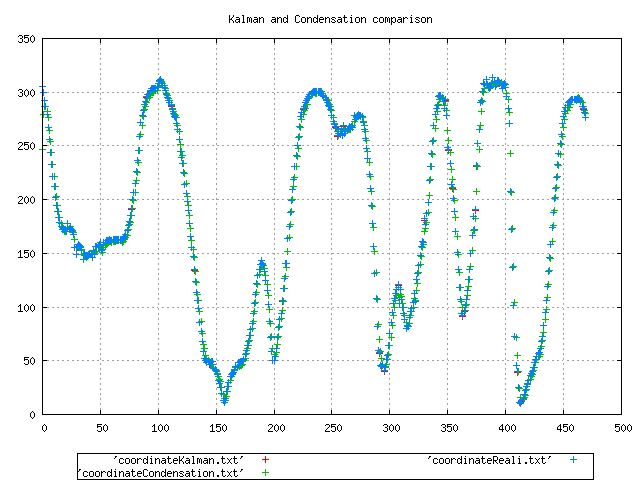
\includegraphics[scale=0.4]{../../esperimenti/tappeto_nozoom/mod_1-Q_500-S_1000/plot.png}
\caption{\textit{Test 10: Tracciamento}}
\end{figure}

\begin{figure}[hb]
\centering
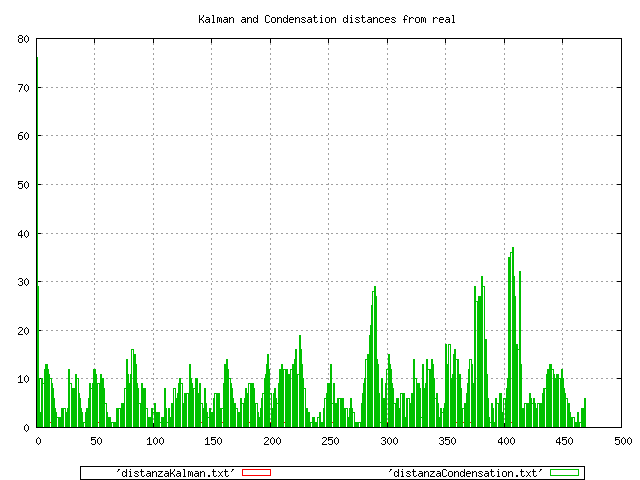
\includegraphics[scale=0.4]{../../esperimenti/tappeto_nozoom/mod_1-Q_500-S_1000/plot-distances.png}
\caption{\textit{Test 10: Previsioni}}
\end{figure}

Statistiche:
\begin{itemize}
\item \begin{math} \bar \delta_K: 0 \end{math}
\item \begin{math} \bar \delta_C: 8 \end{math}
\item \begin{math}(\sigma_x,\sigma_y)\end{math}: (55,41)
\end{itemize}

Anche diminuendo l'area dell'ellisse di tolleranza per Kalman i risultati non cambiano

\newpage
\subsection{Video: singlecar.avi}

\begin{itemize}
\item risoluzione: 648x484
\item fps: 30.00
\item durata: 33 s
\end{itemize}

Anche in questo caso il video è di un'automobilina radiocomadata ripresa dall'alto trasversalmente. A differenza che negli altri video non ci sono oggetti occludenti e il moto è piuttosto uniforme. L'automobilina, però, entra ed esce dalla scena più di una volta.

\begin{figure}[hb]
\centering
	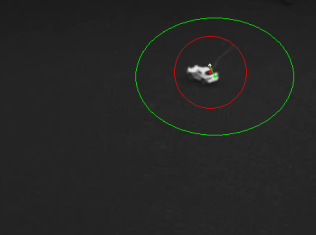
\includegraphics[scale=0.5]{singlecar.png}
\caption{\textit{movie12 screenshot}}
\end{figure}

\newpage
\subsubsection{Test 11: MOD=3, Q=1000, S=1000}

\begin{figure}[hb]
\centering
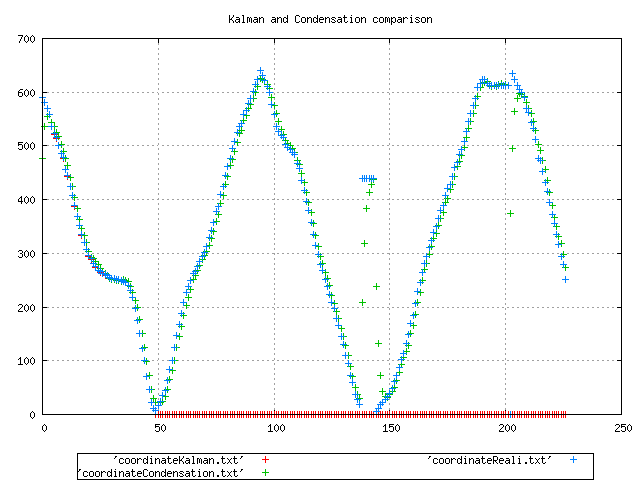
\includegraphics[scale=0.4]{../../esperimenti/single_car/mod_3-Q_1000-S_1000/plot.png}
\caption{\textit{Test 11: Tracciamento}}
\end{figure}

\begin{figure}[hb]
\centering
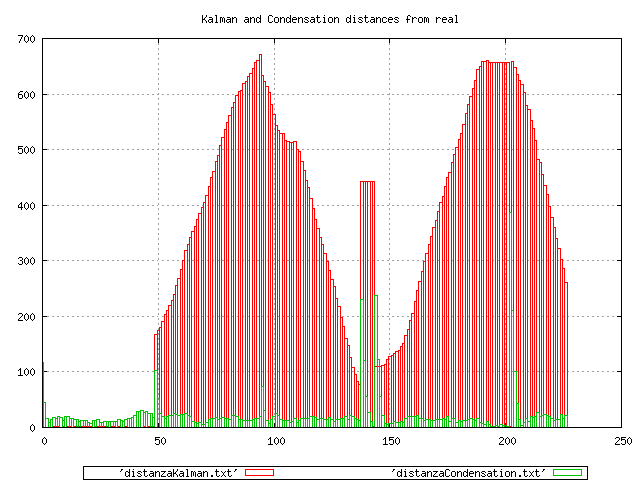
\includegraphics[scale=0.4]{../../esperimenti/single_car/mod_3-Q_1000-S_1000/plot-distances.png}
\caption{\textit{Test 11: Previsioni}}
\end{figure}

Statistiche:
\begin{itemize}
\item \begin{math} \bar \delta_K: 323  \end{math}
\item \begin{math} \bar \delta_C: 23 \end{math}
\item \begin{math}(\sigma_x,\sigma_y)\end{math}: (111,83)
\end{itemize}

In questo test si hanno i risultati più comuni: se l'oggetto scompare dalle scena e riappare in punti molto distanti da dove è scomparso il filtro di Kalman lo perde, ma quando l'oggetto è individuato correttamente Kalman è migliore del Condensation. 

\newpage
\subsubsection{Test 12: MOD=10, Q=5000, S=1000}

\begin{figure}[hb]
\centering
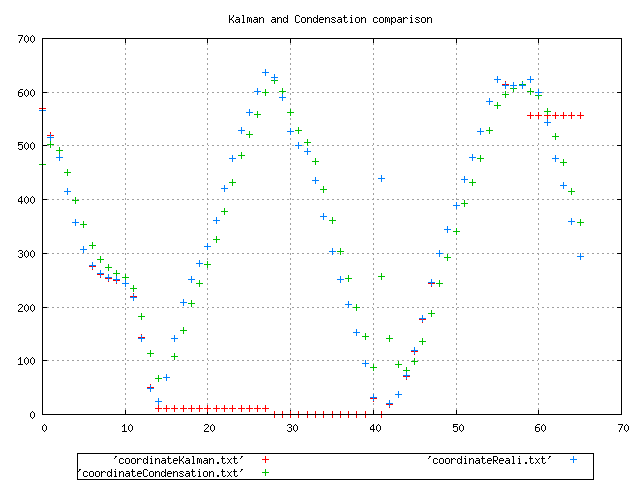
\includegraphics[scale=0.4]{../../esperimenti/single_car/mod_10-Q_5000-S_1000/plot.png}
\caption{\textit{Test 12: Tracciamento}}
\end{figure}

\begin{figure}[hb]
\centering
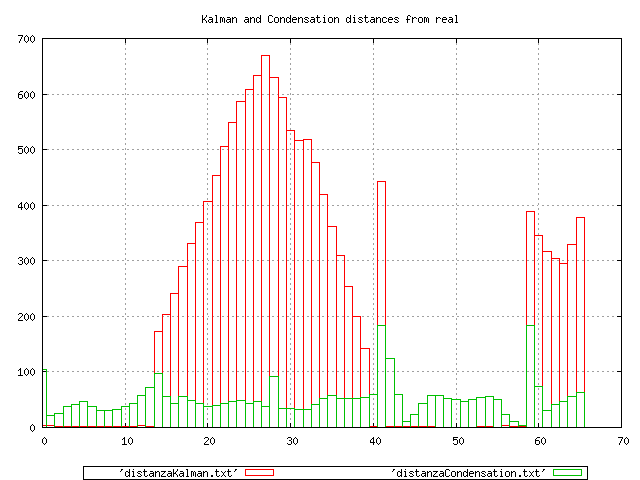
\includegraphics[scale=0.4]{../../esperimenti/single_car/mod_10-Q_5000-S_1000/plot-distances.png}
\caption{\textit{Test 12: Previsioni}}
\end{figure}

Statistiche:
\begin{itemize}
\item \begin{math} \bar \delta_K:  209 \end{math}
\item \begin{math} \bar \delta_C:  52 \end{math}
\item \begin{math}(\sigma_x,\sigma_y)\end{math}: (114,83)
\end{itemize}

Il video in questione si presta ad un tracciamento effettuato ad intervalli più ampi poichè non ci sono brusche accelerazioni o frenate. Il problema principale sul filtro di Kalman resta ed è perciò evidente la necessità di incrementare l'area di tolleranza per migliorare le prestazioni del filtro. 

\newpage
\subsubsection{Test 13: MOD=6, Q=1000, S=1000}

\begin{figure}[hb]
\centering
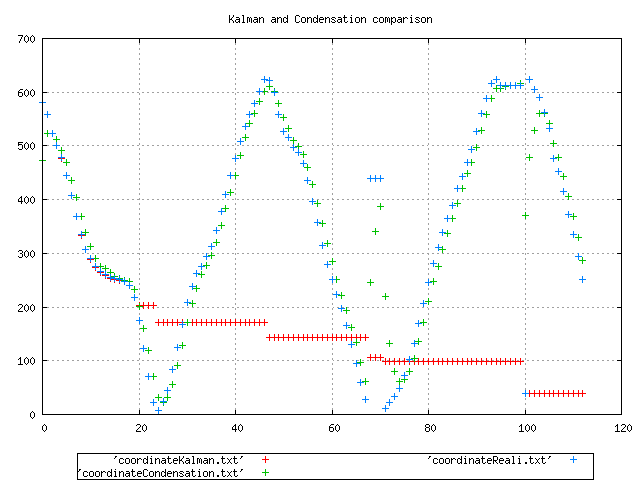
\includegraphics[scale=0.4]{../../esperimenti/single_car/mod_6-Q_1000-S_1000/plot.png}
\caption{\textit{Test 13: Tracciamento}}
\end{figure}

\begin{figure}[hb]
\centering
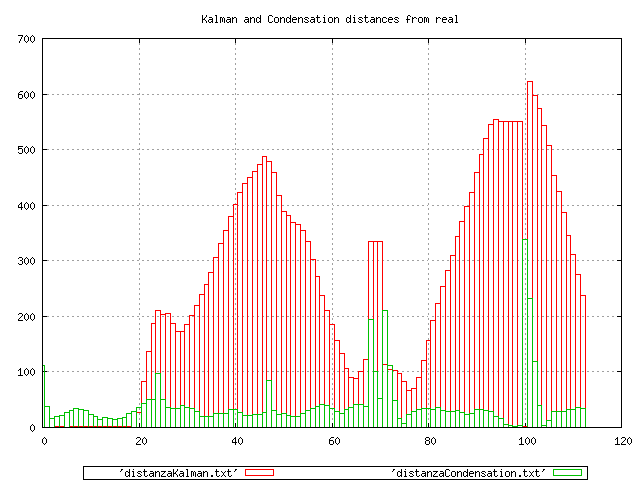
\includegraphics[scale=0.4]{../../esperimenti/single_car/mod_6-Q_1000-S_1000/plot-distances.png}
\caption{\textit{Test 13: Previsioni}}
\end{figure}

Statistiche:
\begin{itemize}
\item \begin{math} \bar \delta_K: 252 \end{math}
\item \begin{math} \bar \delta_C: 40 \end{math}
\item \begin{math}(\sigma_x,\sigma_y)\end{math}: (113,82)
\end{itemize}

Anche riducendo in numero di frames di campionamento la situazione non cambia molto, anzi per un caso crediamo dovuto alla natura del video la situazione addirittura peggiora per Kalman.
Decidiamo perciò di togliere il controllo sulla correttezza del rilevamento da parte di Kalman e costringiamo questo a lavorare nelle condizionidi minima tolleranza sull'errore.

\newpage
\subsubsection{Test 14: MOD=6, Q=1, S=1000}

\begin{figure}[hb]
\centering
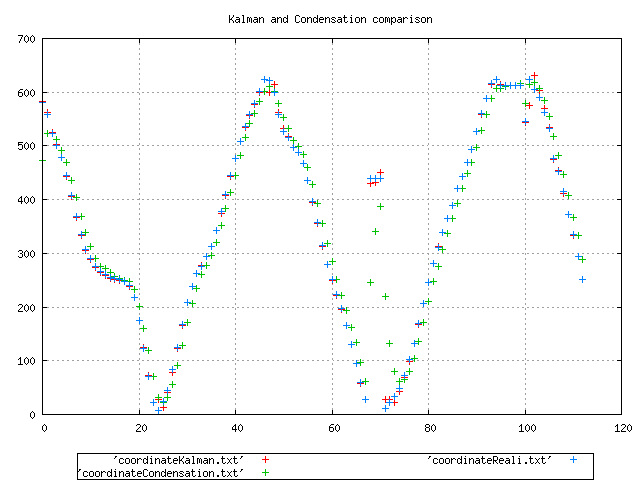
\includegraphics[scale=0.4]{../../esperimenti/single_car/mod_6-Q_1-S_1000/plot.png}
\caption{\textit{Test 14: Tracciamento}}
\end{figure}

\begin{figure}[hb]
\centering
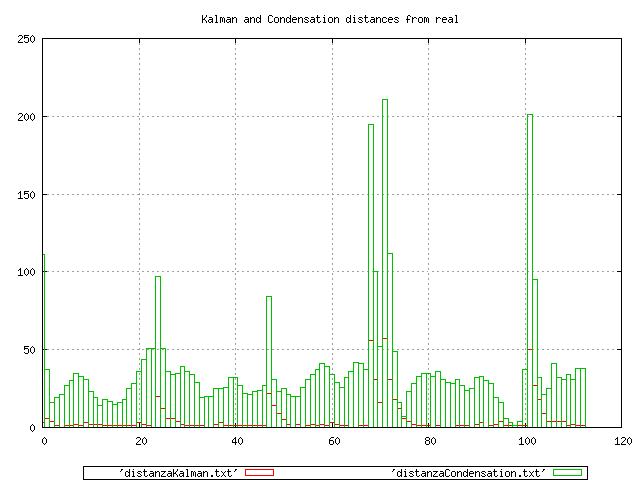
\includegraphics[scale=0.4]{../../esperimenti/single_car/mod_6-Q_1-S_1000/plot-distances.png}
\caption{\textit{Test 14: Previsioni}}
\end{figure}

Statistiche:
\begin{itemize}
\item \begin{math} \bar \delta_K: 5 \end{math}
\item \begin{math} \bar \delta_C: 37 \end{math}
\item \begin{math}(\sigma_x,\sigma_y)\end{math}: (113,82)
\end{itemize}

Il comportamento è più o meno il solito, solo che togliendo il controllo sul rilevamento corretto da parte di Kalman, se l'oggetto scompare siamo comuque in grado di tracciarlo, il filtro di Kalman lo ''insegue''. 
L'obiettivo è ora quello di metterci in una situazione ipotetica in cui Kalman si comporta peggio del Condensation.

\newpage
\subsubsection{Test 15: MOD=6, Q=0.1, S=1000}

\begin{figure}[hb]
\centering
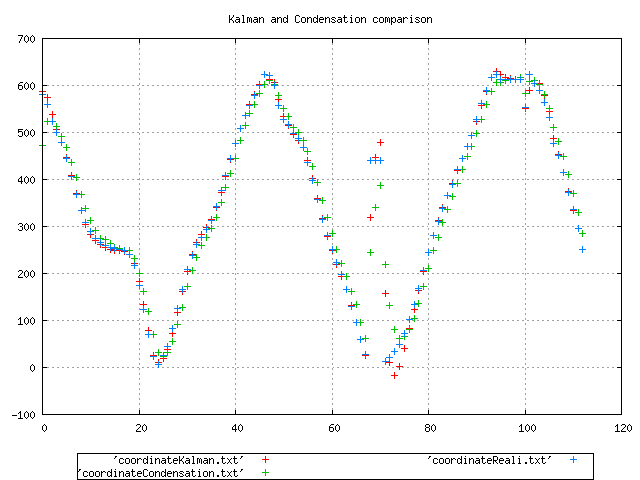
\includegraphics[scale=0.4]{../../esperimenti/single_car/mod_6-Q_0.1-S_1000/plot.png}
\caption{\textit{Test 15: Tracciamento}}
\end{figure}

\begin{figure}[hb]
\centering
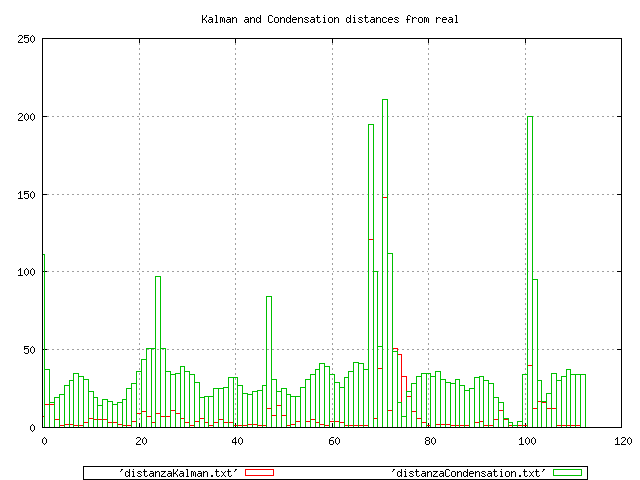
\includegraphics[scale=0.4]{../../esperimenti/single_car/mod_6-Q_0.1-S_1000/plot-distances.png}
\caption{\textit{Test 15: Previsioni}}
\end{figure}

Statistiche:
\begin{itemize}
\item \begin{math} \bar \delta_K: 8 \end{math}
\item \begin{math} \bar \delta_C: 37 \end{math}
\item \begin{math}(\sigma_x,\sigma_y)\end{math}: (113,82)
\end{itemize}

\newpage
\subsubsection{Test 16: MOD=6, Q=0.001, S=1000}

\begin{figure}[hb]
\centering
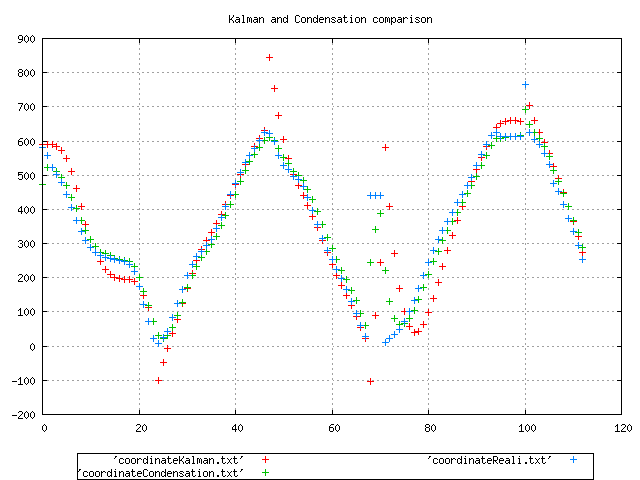
\includegraphics[scale=0.4]{../../esperimenti/single_car/mod_6-Q_0.001-S_1000/plot.png}
\caption{\textit{Test 16: Tracciamento}}
\end{figure}

\begin{figure}[hb]
\centering
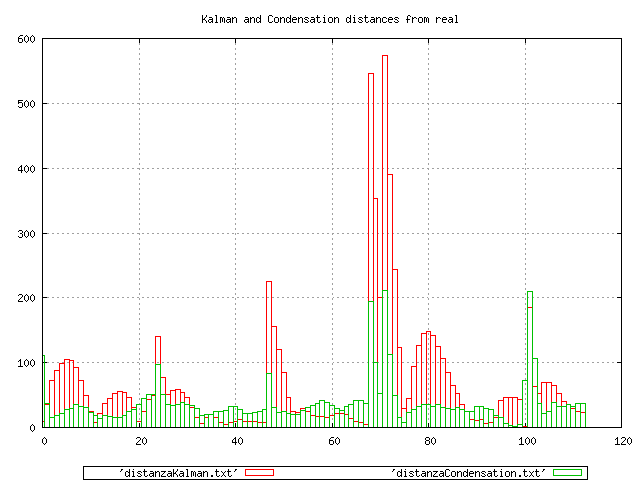
\includegraphics[scale=0.4]{../../esperimenti/single_car/mod_6-Q_0.001-S_1000/plot-distances.png}
\caption{\textit{Test 16: Previsioni}}
\end{figure}

Statistiche:
\begin{itemize}
\item \begin{math} \bar \delta_K: 66 \end{math}
\item \begin{math} \bar \delta_C: 82 \end{math}
\item \begin{math}(\sigma_x,\sigma_y)\end{math}: (114,82)
\end{itemize}

Come previsto il filtro di Kalman comincia a peggiorare il proprio comportamento. 

\newpage
\subsubsection{Test 17: MOD=6, Q=0.0001, S=1000}

\begin{figure}[hb]
\centering
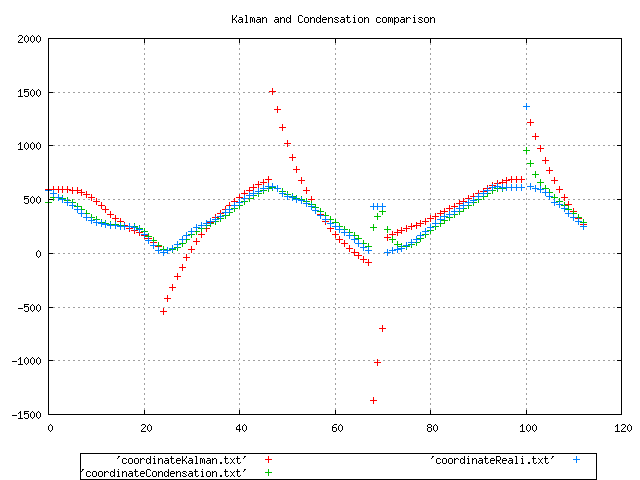
\includegraphics[scale=0.4]{../../esperimenti/single_car/mod_6-Q_0.0001-S_1000/plot.png}
\caption{\textit{Test 17: Tracciamento}}
\end{figure}

\begin{figure}[hb]
\centering
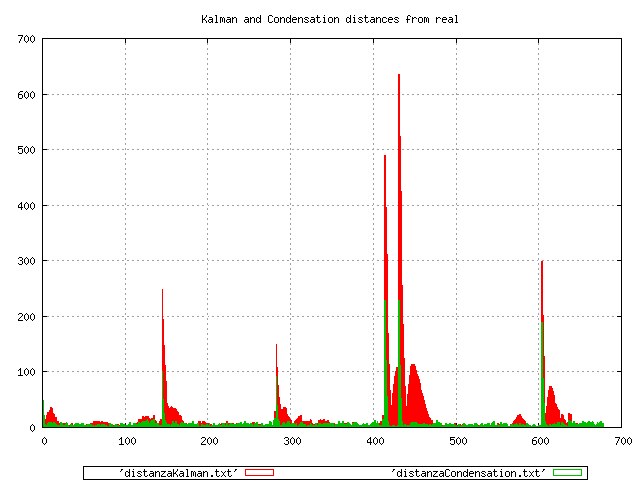
\includegraphics[scale=0.4]{../../esperimenti/single_car/mod_1-Q_0.0001-S_1000/plot-distances.png}
\caption{\textit{Test 17: Previsioni}}
\end{figure}

Statistiche:
\begin{itemize}
\item \begin{math} \bar \delta_K: 179 \end{math}
\item \begin{math} \bar \delta_C: 43 \end{math}
\item \begin{math}(\sigma_x,\sigma_y)\end{math}: (114,83)
\end{itemize}

Kalman non riesce più a tracciare correttamente l'oggetto.

\newpage
\subsubsection{Test 18: MOD=1, Q=0.0001, S=1000}

\begin{figure}[hb]
\centering
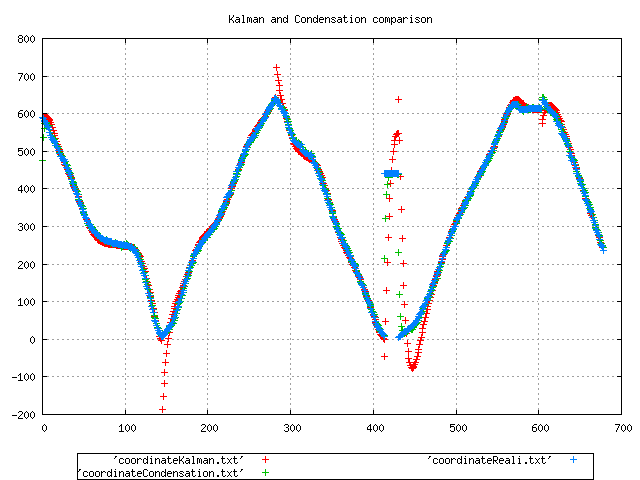
\includegraphics[scale=0.4]{../../esperimenti/single_car/mod_1-Q_0.0001-S_1000/plot.png}
\caption{\textit{Test 18: Tracciamento}}
\end{figure}

\begin{figure}[hb]
\centering
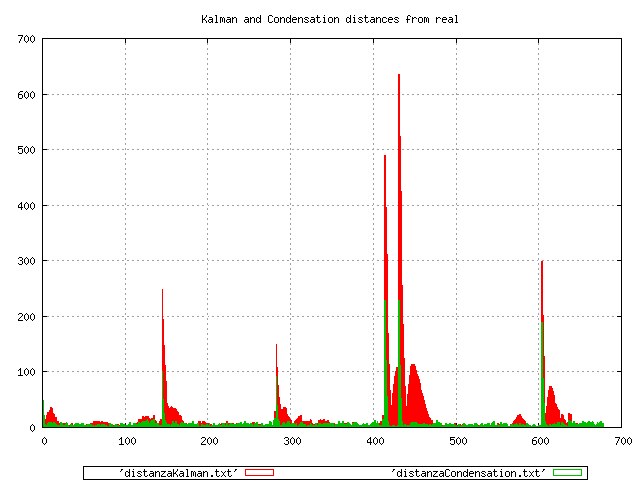
\includegraphics[scale=0.4]{../../esperimenti/single_car/mod_1-Q_0.0001-S_1000/plot-distances.png}
\caption{\textit{Test 18: Previsioni}}
\end{figure}

Qui il comportamento di Kalman è migliore rispetto a prima, questo rende più evidente come Kalman si trovi in difficoltà soprattutto nel tracciare zone di non linearità del moto dell'oggetto. (smoothness)

Statistiche:
\begin{itemize}
\item \begin{math} \bar \delta_K:  \end{math}
\item \begin{math} \bar \delta_C:  \end{math}
\item \begin{math}(\sigma_x,\sigma_y)\end{math}: (,)
\end{itemize}

